\documentclass{tufte-handout}
\usepackage{pgfplots}
\usepackage[dvipsnames]{xcolor}
\usepackage{amsmath, amssymb, amsthm}
\usepackage{mathtools}
\usepackage{bm}
\usepackage{thmtools}
\usepackage{enumitem}
\usepackage{algorithm}
\usepackage{algpseudocode}
\usepackage{tikz}
\usetikzlibrary{calc,arrows.meta,positioning}

% Color scheme (matching your existing document)
\definecolor{wp-bg}{HTML}{FDF6EF}
\definecolor{wp-text}{HTML}{2D1B0E}
\definecolor{wp-primary}{HTML}{C24A3A}
\definecolor{wp-accent}{HTML}{D4952E}
\definecolor{wp-light}{HTML}{F0DECA}
\definecolor{wp-muted}{HTML}{C4A88A}
\definecolor{wp-dark}{HTML}{1A0F07}

\pagecolor{wp-bg}
\color{wp-text}
\hypersetup{colorlinks=true,linkcolor=wp-primary,urlcolor=wp-accent}

% Theorem environments
\declaretheorem[style=plain, name=Definition, numberwithin=section]{defn}
\declaretheorem[style=plain, name=Theorem, numberwithin=section]{thm}
\declaretheorem[style=plain, name=Lemma, numberwithin=section]{lem}
\declaretheorem[style=remark, name=Example, numberwithin=section]{exmp}
\declaretheorem[style=remark, name=Remark, numberwithin=section]{remark}

\title{Recurrent Neural Networks \\ Mathematical Foundations}
\author{Vitor N. Cabral de Oliveira\\ \href{mailto:vnco@cin.ufpe.br}{vnco@cin.ufpe.br}}
\date{\today}

\begin{document}

\maketitle

\begin{abstract}
    This chapter develops the mathematical framework for Recurrent Neural Networks (RNNs), which are designed to process sequential data. We formalise the RNN architecture, derive the forward propagation equations, and present backpropagation through time (BPTT). The problems of vanishing and exploding gradients are analysed, and the Long Short‑Term Memory (LSTM) and Gated Recurrent Unit (GRU) are introduced as effective solutions.
\end{abstract}

\newpage
\hypersetup{linkcolor=wp-text}
\tableofcontents
\hypersetup{linkcolor=wp-primary}
\newpage

\section{Foundations of Sequence Modeling}

Before diving into recurrent architectures, we must establish a rigorous framework for sequence data. Sequences are ordered collections of observations that arise naturally in time series, natural language, audio, video, and many other domains. Understanding their structure and the associated learning problems is essential.

\subsection{Definition and Notation}

\begin{defn}[Sequence]
    A \textbf{sequence} of length $T$ is an ordered tuple $\mathbf{x}_{1:T} = (\mathbf{x}_1, \mathbf{x}_2, \dots, \mathbf{x}_T)$, where each element $\mathbf{x}_t$ belongs to a set $\mathcal{X}$ (the \textbf{observation space}). When $\mathcal{X} \subseteq \mathbb{R}^d$, we speak of a \textbf{real‑valued vector sequence}. 
    \begin{itemize}
        \item If $T$ is finite, the sequence is \textbf{finite}; if $T = \infty$, it is \textbf{infinite}.
        \item When the indices $t$ are discrete (e.g., $t \in \mathbb{N}$), we have a \textbf{discrete‑time sequence}. Continuous‑time sequences are indexed by $t \in \mathbb{R}$ but are less common in machine learning.
    \end{itemize}
\end{defn}

\begin{marginfigure}
\centering
\begin{tikzpicture}[scale=0.8]
    \begin{axis}[width=4cm, height=2.5cm, xlabel=$t$, ylabel=$x_t$, domain=0:10, samples=100, axis lines=middle, enlargelimits]
        \addplot[wp-primary, thick] {sin(deg(x)) + 0.2*rand};
    \end{axis}
    \caption{A real‑valued discrete‑time sequence (time series).}
\end{tikzpicture}
\end{marginfigure}

\paragraph{Special cases}
\begin{itemize}
    \item \textbf{Univariate sequence}: each $\mathbf{x}_t \in \mathbb{R}$ (scalar). Example: daily temperature.
    \item \textbf{Multivariate sequence}: each $\mathbf{x}_t \in \mathbb{R}^d$, $d>1$. Example: joint angles of a robotic arm over time.
    \item \textbf{Symbolic sequence}: $\mathcal{X}$ is a finite set of symbols (e.g., characters, words). Example: natural language text.
\end{itemize}

\subsection{Probabilistic Description}

A sequence can be modelled as a \textbf{stochastic process} $\{X_t\}_{t \in \mathcal{T}}$, where each $X_t$ is a random variable taking values in $\mathcal{X}$, and $\mathcal{T}$ is the index set (usually $\mathbb{N}$ or $\{1,\dots,T\}$). The joint distribution over the entire sequence is $P(X_1 = x_1, \dots, X_T = x_T)$.

\begin{defn}[Stationarity]
    A stochastic process is \textbf{strictly stationary} if for any $t_1,\dots,t_k$ and any shift $\tau$,
    \[
    P(X_{t_1} \le x_1, \dots, X_{t_k} \le x_k) = P(X_{t_1+\tau} \le x_1, \dots, X_{t_k+\tau} \le x_k).
    \]
    It is \textbf{weakly stationary} (or covariance stationary) if:
    \begin{enumerate}
        \item $\mathbb{E}[X_t] = \mu$ (constant mean),
        \item $\operatorname{Var}(X_t) = \sigma^2$ (constant variance),
        \item $\operatorname{Cov}(X_t, X_{t+\tau})$ depends only on $\tau$ (the lag).
    \end{enumerate}
\end{defn}

Stationarity simplifies modeling because the statistical properties do not change over time. Many real‑world sequences are non‑stationary (e.g., financial returns have time‑varying volatility).

\subsection{Auto‑correlation and Memory}

A key characteristic of sequences is that observations are not independent; they exhibit \textbf{temporal dependence}.

\begin{defn}[Auto‑correlation Function (ACF)]
    For a weakly stationary sequence with variance $\sigma^2$, the auto‑correlation at lag $\tau$ is
    \[
    \rho(\tau) = \frac{\operatorname{Cov}(X_t, X_{t+\tau})}{\sigma^2}.
    \]
    The ACF satisfies $\rho(0)=1$, $|\rho(\tau)|\le 1$, and $\rho(\tau)=\rho(-\tau)$.
\end{defn}

If $\rho(\tau)$ decays slowly (e.g., $\rho(\tau) \sim e^{-\alpha \tau}$ or power‑law), the sequence has \textbf{long‑term memory}. Short‑memory processes have $\rho(\tau) \to 0$ exponentially fast.

\begin{marginfigure}
\centering
\begin{tikzpicture}[scale=0.7]
    \begin{axis}[width=4cm, height=2.5cm, xlabel=$\tau$, ylabel=$\rho(\tau)$, domain=0:10, samples=50, axis lines=middle, enlargelimits]
        \addplot[wp-primary, thick] {exp(-0.5*x)};
        \addplot[wp-accent, thick] {0.8^abs(x)};
        \legend{fast decay, slow decay};
    \end{axis}
    \caption{Auto‑correlation functions: exponential (fast) vs. power‑law (slow).}
\end{tikzpicture}
\end{marginfigure}

\subsection{Markov Property and Order}

A fundamental simplification for sequence modeling is the Markov assumption: the future depends only on a finite past.

\begin{defn}[Markov Chain]
    A discrete‑time stochastic process $\{X_t\}$ is a \textbf{Markov chain of order $k$} if for all $t$,
    \[
    P(X_t = x_t \mid X_{1:t-1} = x_{1:t-1}) = P(X_t = x_t \mid X_{t-k:t-1} = x_{t-k:t-1}),
    \]
    i.e., the conditional distribution of the next state depends only on the $k$ most recent states. For $k=1$, it is a \textbf{first‑order Markov chain}.
\end{defn}

\begin{thm}[Markov Chain Decomposition]
    For a first‑order Markov chain, the joint distribution factorizes as
    \[
    P(X_{1:T} = x_{1:T}) = P(X_1 = x_1) \prod_{t=2}^{T} P(X_t = x_t \mid X_{t-1} = x_{t-1}).
    \]
\end{thm}

The Markov property is the theoretical backbone of many sequence models, including RNNs (which approximate an infinite‑order Markov chain via hidden states).

\subsection{Deep Dive: Markov Models}

\paragraph{Discrete‑Time Markov Chains}
A discrete‑time stochastic process $\{X_t\}_{t=1}^\infty$ with state space $\mathcal{S}$ (finite or countable) is a \textbf{Markov chain} if for all $t \ge 2$ and all $s_1,\dots,s_t \in \mathcal{S}$,
\[
P(X_t = s_t \mid X_{t-1}=s_{t-1}, \dots, X_1=s_1) = P(X_t = s_t \mid X_{t-1}=s_{t-1}).
\]
The chain is \textbf{time‑homogeneous} if the transition probability does not depend on $t$:
\[
P(X_t = j \mid X_{t-1}=i) = T_{ij}, \quad \forall t,
\]
where $\mathbf{T}$ is the \textbf{transition matrix} with rows summing to $1$.

\begin{marginfigure}
\centering
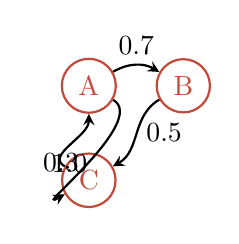
\begin{tikzpicture}[node distance=1.2cm, thick, >=stealth]
    \node[draw, circle, wp-primary] (A) {A};
    \node[draw, circle, wp-primary, right of=A] (B) {B};
    \node[draw, circle, wp-primary, below of=A] (C) {C};
    \draw[->] (A) to[out=30,in=150] node[above] {$0.7$} (B);
    \draw[->] (A) to[out=-30,in=-150] node[left] {$0.3$} (C);
    \draw[->] (B) to[out=210,in=30] node[right] {$0.5$} (C);
    \draw[->] (C) to[out=150,in=-90] node[below] {$1.0$} (A);
\end{tikzpicture}
\caption{A three‑state Markov chain with transition probabilities.}
\end{marginfigure}

\begin{defn}[Order $k$ Markov Chain]
    A process satisfies the \textbf{Markov property of order $k$} if
    \[
    P(X_t \mid X_{1:t-1}) = P(X_t \mid X_{t-k:t-1}).
    \]
    The state can be augmented to $\tilde{X}_t = (X_{t-k+1}, \dots, X_t)$, which forms a first‑order chain on a larger state space of size $|\mathcal{S}|^k$.
\end{defn}

\paragraph{Key Properties of Markov Chains}
\begin{itemize}
    \item \textbf{Stationary distribution}: If a distribution $\boldsymbol{\pi}$ satisfies $\boldsymbol{\pi}^{\mathsf{T}} = \boldsymbol{\pi}^{\mathsf{T}} \mathbf{T}$, it is stationary; for an ergodic chain, $\lim_{n\to\infty} \mathbf{T}^n$ has rows equal to $\boldsymbol{\pi}$.
    \item \textbf{Ergodicity}: A chain that is aperiodic and positive recurrent converges to a unique stationary distribution regardless of initial state.
    \item \textbf{Likelihood of a sequence}: $P(X_{1:T}=s_{1:T}) = P(X_1=s_1) \prod_{t=2}^T T_{s_{t-1}, s_t}$.
\end{itemize}

\paragraph{Hidden Markov Models (HMMs)}
In many real‑world sequences, the underlying state is not directly observable. HMMs extend Markov chains by assuming that each state $X_t$ emits an observation $O_t$ through a known emission distribution.

\begin{defn}[Hidden Markov Model]
    An HMM is a doubly stochastic process $(X_t, O_t)_{t=1}^T$ where:
    \begin{enumerate}
        \item $\{X_t\}$ is a time‑homogeneous Markov chain with state space $\mathcal{S}$, initial distribution $\boldsymbol{\pi}$, and transition matrix $\mathbf{T}$.
        \item Given $X_t$, the observation $O_t$ is independent of all other states and observations, with emission probability $E(o \mid X_t=s) = P(O_t=o \mid X_t=s)$.
    \end{enumerate}
    The joint distribution of a sequence of states and observations is
    \[
    P(X_{1:T}=s_{1:T}, O_{1:T}=o_{1:T}) = \pi_{s_1} \prod_{t=2}^T T_{s_{t-1}, s_t} \prod_{t=1}^T E(o_t \mid s_t).
    \]
\end{defn}

\begin{marginfigure}
\centering
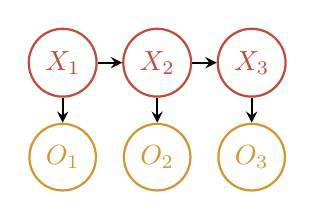
\begin{tikzpicture}[node distance=1.2cm, thick, >=stealth]
    \node[draw, circle, wp-primary] (X1) {$X_1$};
    \node[draw, circle, wp-primary, right of=X1] (X2) {$X_2$};
    \node[draw, circle, wp-primary, right of=X2] (X3) {$X_3$};
    \draw[->] (X1) -- (X2);
    \draw[->] (X2) -- (X3);
    \node[draw, circle, wp-accent, below of=X1] (O1) {$O_1$};
    \node[draw, circle, wp-accent, below of=X2] (O2) {$O_2$};
    \node[draw, circle, wp-accent, below of=X3] (O3) {$O_3$};
    \draw[->] (X1) -- (O1);
    \draw[->] (X2) -- (O2);
    \draw[->] (X3) -- (O3);
\end{tikzpicture}
\caption{Graphical model of an HMM: hidden states $X_t$ (circle) emit observations $O_t$ (square).}
\end{marginfigure}

\paragraph{Inference and Learning in HMMs}
Three fundamental problems for HMMs are solved with efficient dynamic programming algorithms.

\emph{1. Likelihood Computation (Forward Algorithm)}
Given observations $o_{1:T}$, compute $P(O_{1:T}=o_{1:T}) = \sum_{s_{1:T}} P(X_{1:T}, O_{1:T})$. The forward recursion:
\[
\alpha_1(s) = \pi_s \, E(o_1 \mid s), \quad
\alpha_t(s) = E(o_t \mid s) \sum_{s'} \alpha_{t-1}(s') \, T_{s', s}.
\]
Then $P(O_{1:T}) = \sum_s \alpha_T(s)$.

\emph{2. Most Likely State Sequence (Viterbi)}
Find $\arg\max_{s_{1:T}} P(X_{1:T} \mid O_{1:T})$. The Viterbi algorithm uses:
\[
\delta_1(s) = \pi_s E(o_1 \mid s),\quad
\delta_t(s) = E(o_t \mid s) \max_{s'} \delta_{t-1}(s') T_{s', s},
\]
with backpointers to reconstruct the optimal path.

\emph{3. Parameter Estimation (Baum–Welch / EM)}
Given observations but no states, we maximise $\log P(O_{1:T} \mid \boldsymbol{\theta})$ via the EM algorithm. The E‑step computes posterior probabilities $\gamma_t(s) = P(X_t=s \mid O_{1:T})$ and $\xi_t(s',s) = P(X_{t-1}=s', X_t=s \mid O_{1:T})$ using the forward–backward algorithm. The M‑step updates:
\[
\pi_s \propto \gamma_1(s),\quad T_{s',s} \propto \frac{\sum_{t=2}^T \xi_t(s',s)}{\sum_{t=2}^T \gamma_{t-1}(s')},\quad
E(o \mid s) \propto \frac{\sum_{t: O_t=o} \gamma_t(s)}{\sum_t \gamma_t(s)}.
\]

\begin{thm}[Baum–Welch Convergence]
    The Baum–Welch algorithm monotonically increases the likelihood $P(O_{1:T} \mid \boldsymbol{\theta})$ and converges to a local maximum of the likelihood.
\end{thm}

\paragraph{Markov Decision Processes (MDPs) – A Brief Mention}
When actions influence state transitions, we obtain an MDP. While not purely generative, MDPs are foundational for reinforcement learning. An MDP is a tuple $(\mathcal{S}, \mathcal{A}, \mathcal{T}, \mathcal{R}, \gamma)$ where:
\begin{itemize}
    \item $\mathcal{S}$: state space,
    \item $\mathcal{A}$: action space,
    \item $\mathcal{T}(s' \mid s, a)$: transition probability,
    \item $\mathcal{R}(s,a)$: immediate reward,
    \item $\gamma \in [0,1]$: discount factor.
\end{itemize}
The goal is to find a policy $\pi(a \mid s)$ that maximises expected cumulative reward.

\paragraph{From Hidden Markov Models to Recurrent Neural Networks}
HMMs and RNNs both address sequence modeling but differ fundamentally:
\begin{itemize}
    \item \textbf{State representation}: HMM states are discrete (finite $\mathcal{S}$); RNN states are continuous vectors $\mathbf{h}_t \in \mathbb{R}^{d_h}$. Continuous states allow exponentially more expressive power for a fixed dimensionality.
    \item \textbf{Transition function}: HMM transitions are linear (matrix multiplication on a simplex); RNN transitions are nonlinear (e.g., $\tanh(\mathbf{W}_{hh}\mathbf{h}_{t-1} + \mathbf{W}_{xh}\mathbf{x}_t)$), enabling the modelling of complex dynamics.
    \item \textbf{Emission model}: HMM emissions factorize as $E(o_t \mid s_t)$; RNNs can produce outputs that depend on the entire history via $\mathbf{h}_t$.
    \item \textbf{Learning}: HMMs are trained with EM (Baum–Welch), which guarantees local likelihood increase; RNNs use BPTT and stochastic gradient descent, which scale better to large state spaces and long sequences.
    \item \textbf{Long‑range dependencies}: HMMs suffer from exponentially many states to represent $k$‑th order dependencies; RNNs attempt to compress history into a fixed‑size vector (though suffer from vanishing gradients).
\end{itemize}

\begin{thm}[HMM as a Linear RNN]
    If the state vector $\mathbf{h}_t$ is taken as the vector of probabilities $P(X_t=s \mid \text{history})$, then the update $\mathbf{h}_t \propto \mathbf{E}_{o_t} \odot (\mathbf{T}^{\mathsf{T}} \mathbf{h}_{t-1})$ (normalised) is a linear recurrence (with a non‑linear normalisation). This is equivalent to the forward algorithm of an HMM.
\end{thm}

The inadequacies of HMMs for large‑scale sequence modeling – discrete state, linear transitions, independence of observations given state – motivated the development of more powerful models, including conditional random fields (CRFs) and ultimately recurrent neural networks. However, HMMs remain important for their interpretability, small‑sample efficiency, and theoretical guarantees.

\begin{marginfigure}
\centering
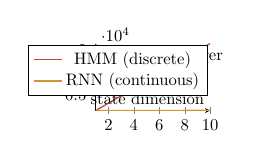
\begin{tikzpicture}[scale=0.6]
    \begin{axis}[width=4cm, height=3cm, xlabel=state dimension, ylabel=expressive power, domain=1:10, samples=2, axis lines=middle]
        \addplot[wp-primary, thick] {exp(x)};
        \addplot[wp-accent, thick] {1.5^x};
        \legend{HMM (discrete), RNN (continuous)};
    \end{axis}
\end{tikzpicture}
\caption{Continuous RNN states can represent exponentially more distinct histories than discrete HMM states of the same dimension.}
\end{marginfigure}

\subsection{Sequence Learning Tasks}

We categorise learning problems based on inputs and outputs:

\begin{enumerate}
    \item \textbf{Sequence prediction (auto‑regressive)}: Given past observations $x_{1:t-1}$, predict $x_t$. The model learns $P(x_t \mid x_{1:t-1})$.
    \item \textbf{Sequence classification}: Given the entire input sequence $\mathbf{x}_{1:T}$, predict a single label $y$. Example: sentiment analysis.
    \item \textbf{Sequence labelling (per‑time‑step classification)}: Given $\mathbf{x}_{1:T}$, predict a label $y_t$ for each $t$. Example: part‑of‑speech tagging.
    \item \textbf{Sequence generation}: Sample a new sequence from the learned distribution $P(x_{1:T})$.
    \item \textbf{Sequence‑to‑sequence (seq2seq)}: Map an input sequence $\mathbf{x}_{1:T}$ to an output sequence $\mathbf{y}_{1:T'}$ (possibly of different length). Example: machine translation.
\end{enumerate}

\subsection{Why Feedforward Networks Fail for Sequences}

Feedforward (multilayer perceptron) networks assume fixed‑length inputs and outputs, and – critically – they treat each input as independent. To process a sequence of length $T$, one could:
\begin{enumerate}
    \item \textbf{Concatenate all elements} into a single $d \times T$ vector. This fails because $T$ is variable and the resulting dimension becomes enormous.
    \item \textbf{Slide a window} of fixed size $w$ over the sequence, using the last $w$ values as input to a feedforward network. This ignores dependencies longer than $w$ (finite memory) and does not share parameters across time positions efficiently.
\end{enumerate}

Moreover, feedforward networks have no built‑in mechanism to handle the sequential order or to maintain a state that evolves over time. They cannot capture the inductive bias that the same transformation applies at each time step (weight sharing) – a property that recurrent networks exploit.

\begin{marginfigure}
\centering
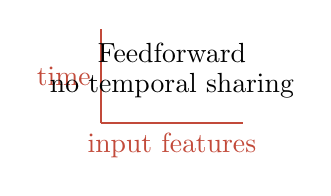
\begin{tikzpicture}[scale=0.6]
    \draw[thick, wp-primary] (0,0) -- (0,2) node[midway, left] {time};
    \draw[thick, wp-primary] (0,0) -- (3,0) node[midway, below] {input features};
    \node at (1.5,1.5) {Feedforward};
    \node at (1.5,0.8) {no temporal sharing};
\end{tikzpicture}
\caption{Feedforward networks treat each time step independently; they cannot share weights across time or maintain a dynamic state.}
\end{marginfigure}

\subsection{Recurrence as a Natural Solution}

An RNN addresses these limitations by introducing a \textbf{hidden state} $\mathbf{h}_t$ that evolves over time according to
\[
\mathbf{h}_t = f(\mathbf{h}_{t-1}, \mathbf{x}_t; \boldsymbol{\theta}),
\]
where $f$ is a parameterised function (same at each step). This gives three crucial properties:
\begin{itemize}
    \item \textbf{Variable‑length handling}: the same recurrence applies for any $T$.
    \item \textbf{Parameter sharing}: the same weights $\boldsymbol{\theta}$ are used at each time step, reducing the number of parameters and promoting generalization.
    \item \textbf{Memory}: the hidden state $\mathbf{h}_t$ can theoretically retain information from arbitrarily distant past (though in practice limited by vanishing gradients).
\end{itemize}

Thus, the RNN is a natural and principled extension of feedforward networks to sequential data. The remainder of this chapter formalises the RNN architecture, training, and its advanced variants.

\section{The Elman RNN Architecture}

The most basic RNN, proposed by Elman (1990), consists of an input layer, a hidden layer with recurrent connections, and an output layer. At each time step $t$, the hidden state $\mathbf{h}_t \in \mathbb{R}^{d_h}$ is updated based on the current input $\mathbf{x}_t$ and the previous hidden state $\mathbf{h}_{t-1}$.

\begin{defn}[RNN Cell]
    A simple RNN cell is defined by the following equations:
    \begin{align}
        \mathbf{a}_t &= \mathbf{W}_{xh} \mathbf{x}_t + \mathbf{W}_{hh} \mathbf{h}_{t-1} + \mathbf{b}_h, \label{eq:rnn_pre} \\
        \mathbf{h}_t &= \phi_h(\mathbf{a}_t), \label{eq:rnn_hidden} \\
        \mathbf{o}_t &= \mathbf{W}_{hy} \mathbf{h}_t + \mathbf{b}_y, \label{eq:rnn_output} \\
        \hat{\mathbf{y}}_t &= \phi_y(\mathbf{o}_t), \label{eq:rnn_pred}
    \end{align}
    where:
    \begin{itemize}
        \item $\mathbf{W}_{xh} \in \mathbb{R}^{d_h \times d_x}$ is the input‑to‑hidden weight matrix,
        \item $\mathbf{W}_{hh} \in \mathbb{R}^{d_h \times d_h}$ is the recurrent (hidden‑to‑hidden) weight matrix,
        \item $\mathbf{W}_{hy} \in \mathbb{R}^{d_y \times d_h}$ is the hidden‑to‑output weight matrix,
        \item $\mathbf{b}_h \in \mathbb{R}^{d_h}$, $\mathbf{b}_y \in \mathbb{R}^{d_y}$ are bias vectors,
        \item $\phi_h$ is a nonlinear activation function (typically $\tanh$ or ReLU),
        \item $\phi_y$ is the output activation (e.g., softmax for classification, identity for regression).
    \end{itemize}
    The initial hidden state $\mathbf{h}_0$ is usually set to the zero vector, but can also be learned.
\end{defn}

\begin{marginfigure}
\centering
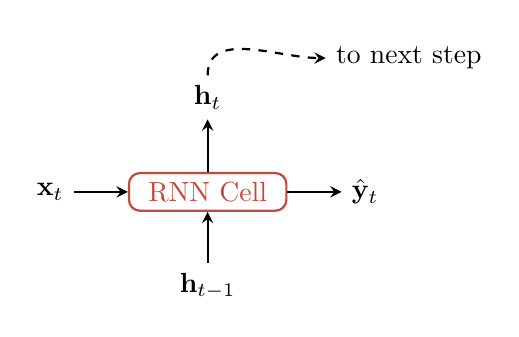
\begin{tikzpicture}[node distance=1cm, thick, >=stealth]
    \node[draw, rectangle, rounded corners, wp-primary, minimum width=2cm] (cell) {RNN Cell};
    \node[left of=cell, node distance=2cm] (x) {$\mathbf{x}_t$};
    \node[below of=cell, node distance=1.2cm] (hprev) {$\mathbf{h}_{t-1}$};
    \node[right of=cell, node distance=2cm] (y) {$\hat{\mathbf{y}}_t$};
    \node[above of=cell, node distance=1.2cm] (h) {$\mathbf{h}_t$};
    \draw[->] (x) -- (cell);
    \draw[->] (hprev) -- (cell);
    \draw[->] (cell) -- (y);
    \draw[->] (cell) -- (h);
    \draw[->, dashed] (h) to[out=90,in=180] ++(1.5,0.5) node[right] {to next step};
\end{tikzpicture}
\caption{Schematic of a single RNN cell. The hidden state $\mathbf{h}_t$ is fed back to the next time step.}
\end{marginfigure}

\subsection{Connection to Linear Dynamical Systems}

Classical state‑space models, known as linear dynamical systems (LDS) or Kalman filters, provide a linear counterpart to RNNs.

\begin{defn}[Linear Dynamical System]
    A discrete‑time LDS is defined by:
    \begin{align}
        \mathbf{h}_t &= \mathbf{A} \mathbf{h}_{t-1} + \mathbf{B} \mathbf{x}_t + \boldsymbol{\epsilon}_t, \quad \boldsymbol{\epsilon}_t \sim \mathcal{N}(0, \mathbf{Q}), \\
        \mathbf{y}_t &= \mathbf{C} \mathbf{h}_t + \boldsymbol{\delta}_t, \quad \boldsymbol{\delta}_t \sim \mathcal{N}(0, \mathbf{R}),
    \end{align}
    where $\mathbf{A}, \mathbf{B}, \mathbf{C}$ are matrices, and $\mathbf{h}_t$ is the latent state.
\end{defn}

Comparing with the Elman RNN:
\[
\mathbf{h}_t = \phi_h(\mathbf{W}_{hh}\mathbf{h}_{t-1} + \mathbf{W}_{xh}\mathbf{x}_t + \mathbf{b}_h).
\]
The RNN generalises the LDS in two ways:
\begin{itemize}
    \item Nonlinear activation $\phi_h$ (instead of identity),
    \item Deterministic state (no process noise), though one can add noise for probabilistic RNNs.
\end{itemize}

If $\phi_h$ is the identity function and $\mathbf{b}_h = \mathbf{0}$, the RNN reduces to a linear system. Conversely, the LDS can be interpreted as a linear RNN with Gaussian noise. Inference in LDS (Kalman smoothing) resembles forward–backward propagation in RNNs but with exact uncertainty propagation. This connection is valuable for understanding RNNs as flexible nonlinear extensions of classical time‑series models.

\begin{marginfigure}
\centering

\begin{tikzpicture}[node distance=1cm, thick]
    \node[draw, rectangle, wp-primary] (rnn) {RNN};
    \node[draw, rectangle, wp-accent, right of=rnn] (lds) {LDS};
    \draw[<->, thick] (rnn) -- node[above] {nonlinear} (lds);
\end{tikzpicture}
\caption{RNNs generalise linear dynamical systems by replacing linear transitions with nonlinear functions.}
\end{marginfigure}

\subsection{Bidirectional Recurrent Neural Networks}

Many sequence tasks – such as part‑of‑speech tagging or named entity recognition – benefit from access to both past and future context. A bidirectional RNN (BiRNN) processes the sequence in two directions.

\begin{defn}[Bidirectional RNN]
    Given an input sequence $\mathbf{x}_{1:T}$, a BiRNN maintains:
    \begin{itemize}
        \item A forward hidden state $\overrightarrow{\mathbf{h}}_t = \text{RNN}_{\text{fwd}}(\mathbf{x}_t, \overrightarrow{\mathbf{h}}_{t-1})$,
        \item A backward hidden state $\overleftarrow{\mathbf{h}}_t = \text{RNN}_{\text{bwd}}(\mathbf{x}_t, \overleftarrow{\mathbf{h}}_{t+1})$,
        \item A combined state $\mathbf{h}_t = [\overrightarrow{\mathbf{h}}_t; \overleftarrow{\mathbf{h}}_t]$ (concatenation) or $\mathbf{h}_t = \overrightarrow{\mathbf{h}}_t + \overleftarrow{\mathbf{h}}_t$.
    \end{itemize}
    The output at time $t$ is computed from $\mathbf{h}_t$: $\hat{\mathbf{y}}_t = \phi_y(\mathbf{W}_y \mathbf{h}_t + \mathbf{b}_y)$.
\end{defn}

\begin{marginfigure}
\centering
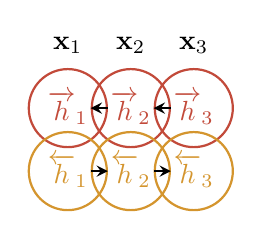
\begin{tikzpicture}[node distance=0.8cm, thick, >=stealth]
    \node[draw, circle, wp-primary] (h1f) {$\overrightarrow{h}_1$};
    \node[draw, circle, wp-primary, right of=h1f] (h2f) {$\overrightarrow{h}_2$};
    \node[draw, circle, wp-primary, right of=h2f] (h3f) {$\overrightarrow{h}_3$};
    \node[draw, circle, wp-accent, below of=h1f] (h1b) {$\overleftarrow{h}_1$};
    \node[draw, circle, wp-accent, right of=h1b] (h2b) {$\overleftarrow{h}_2$};
    \node[draw, circle, wp-accent, right of=h2b] (h3b) {$\overleftarrow{h}_3$};
    \draw[->] (h1f) -- (h2f); \draw[->] (h2f) -- (h3f);
    \draw[<-] (h1b) -- (h2b); \draw[<-] (h2b) -- (h3b);
    \node[above of=h1f] {$\mathbf{x}_1$}; \node[above of=h2f] {$\mathbf{x}_2$}; \node[above of=h3f] {$\mathbf{x}_3$};
\end{tikzpicture}
\caption{Bidirectional RNN: forward (top) and backward (bottom) states are combined.}
\end{marginfigure}

During training, we unroll both directions and compute the loss at each step. Backpropagation through time propagates gradients separately through the forward and backward chains, and the concatenated state gradients are summed. Bidirectional RNNs are not suitable for real‑time or online tasks (since the full sequence is required to compute backward states), but they are very effective for offline sequence labelling.

\subsection{Deep (Stacked) Recurrent Neural Networks}

To increase representational capacity, multiple RNN layers can be stacked vertically. At each time step $t$, the output of layer $\ell-1$ becomes the input to layer $\ell$.

\begin{defn}[Stacked RNN]
    Let $\mathbf{h}_t^{(\ell)}$ denote the hidden state of layer $\ell$ at time $t$, with $\mathbf{h}_t^{(0)} = \mathbf{x}_t$. For $\ell = 1,\dots,L$,
    \[
    \mathbf{a}_t^{(\ell)} = \mathbf{W}_{xh}^{(\ell)} \mathbf{h}_t^{(\ell-1)} + \mathbf{W}_{hh}^{(\ell)} \mathbf{h}_{t-1}^{(\ell)} + \mathbf{b}_h^{(\ell)},\quad
    \mathbf{h}_t^{(\ell)} = \phi_h(\mathbf{a}_t^{(\ell)}).
    \]
    The output is then $\hat{\mathbf{y}}_t = \phi_y(\mathbf{W}_{hy} \mathbf{h}_t^{(L)} + \mathbf{b}_y)$.
\end{defn}

Training deep RNNs requires backpropagation through both time and layers. The gradient flows downwards through the layer hierarchy and backwards in time. Vanishing gradients are exacerbated with depth, so gated architectures (LSTM, GRU) are typically used in deep stacks. Residual connections (skip connections across layers) can also help.

\begin{algorithm}[h]
    \caption{Forward pass for a stacked RNN (2 layers)}
    \begin{algorithmic}[1]
        \State $\mathbf{h}_0^{(1)} \gets \mathbf{0}$, $\mathbf{h}_0^{(2)} \gets \mathbf{0}$
        \For{$t = 1$ to $T$}
            \State $\mathbf{a}_t^{(1)} = \mathbf{W}_{xh}^{(1)}\mathbf{x}_t + \mathbf{W}_{hh}^{(1)}\mathbf{h}_{t-1}^{(1)} + \mathbf{b}_h^{(1)}$
            \State $\mathbf{h}_t^{(1)} = \phi_h(\mathbf{a}_t^{(1)})$
            \State $\mathbf{a}_t^{(2)} = \mathbf{W}_{xh}^{(2)}\mathbf{h}_t^{(1)} + \mathbf{W}_{hh}^{(2)}\mathbf{h}_{t-1}^{(2)} + \mathbf{b}_h^{(2)}$
            \State $\mathbf{h}_t^{(2)} = \phi_h(\mathbf{a}_t^{(2)})$
            \State $\hat{\mathbf{y}}_t = \phi_y(\mathbf{W}_{hy}\mathbf{h}_t^{(2)} + \mathbf{b}_y)$
        \EndFor
    \end{algorithmic}
\end{algorithm}

Deep RNNs are used in applications such as acoustic modelling for speech recognition and machine translation, where hierarchical feature extraction is beneficial.

\subsection{Unrolling Through Time}

To understand training, it is convenient to “unroll” the recurrence over time, obtaining a deep feedforward network with shared weights across layers (each layer corresponds to a time step). The unrolled architecture for $T$ time steps is shown in Figure~\ref{fig:rnn_unrolled}.

\begin{figure}[h]
\centering
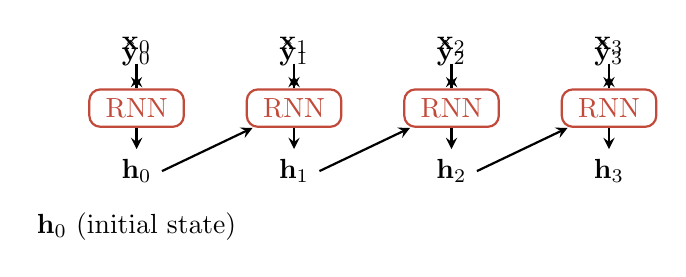
\begin{tikzpicture}[node distance=1cm, thick, >=stealth]
    \foreach \t in {0,1,2,3} {
        \pgfmathsetmacro{\prev}{\t-1}
        \node[draw, rectangle, rounded corners, wp-primary, minimum width=1.2cm] (cell\t) at (\t*2,0) {RNN};
        \node[above of=cell\t, node distance=0.8cm] (x\t) {$\mathbf{x}_\t$};
        \draw[->] (x\t) -- (cell\t);
        \node[below of=cell\t, node distance=0.8cm] (h\t) {$\mathbf{h}_\t$};
        \draw[->] (cell\t) -- (h\t);
        \node[above of=h\t, node distance=1.5cm] (y\t) {$\hat{\mathbf{y}}_\t$};
        \draw[->] (cell\t) -- (y\t);
        \ifnum\t>0
            \draw[->] (h\prev) -- (cell\t);
        \fi
    }
    \node at (0, -1.5) {$\mathbf{h}_0$ (initial state)};
\end{tikzpicture}
\caption{Unrolled RNN for $T=4$ time steps. The same weights $\mathbf{W}_{xh}, \mathbf{W}_{hh}, \mathbf{W}_{hy}$ are reused at every step.}
\label{fig:rnn_unrolled}
\end{figure}

\subsection{Forward Propagation}

Given an input sequence $\mathbf{x}_{1:T}$, forward propagation computes the hidden states and outputs sequentially:

\begin{algorithm}[h]
    \caption{Forward pass of an RNN}
    \begin{algorithmic}[1]
        \State $\mathbf{h}_0 \gets \mathbf{0}$ (or learned initial state)
        \For{$t = 1$ to $T$}
            \State $\mathbf{a}_t \gets \mathbf{W}_{xh}\mathbf{x}_t + \mathbf{W}_{hh}\mathbf{h}_{t-1} + \mathbf{b}_h$
            \State $\mathbf{h}_t \gets \phi_h(\mathbf{a}_t)$
            \State $\mathbf{o}_t \gets \mathbf{W}_{hy}\mathbf{h}_t + \mathbf{b}_y$
            \State $\hat{\mathbf{y}}_t \gets \phi_y(\mathbf{o}_t)$
        \EndFor
    \end{algorithmic}
\end{algorithm}

\section{Training RNNs: Backpropagation Through Time (BPTT)}

RNNs are trained by minimising a loss function that aggregates errors over all time steps. For a sequence with targets $\mathbf{y}_{1:T}$, the total loss is the sum of per‑time‑step losses:
\[
\mathcal{L}(\mathbf{y}_{1:T}, \hat{\mathbf{y}}_{1:T}) = \sum_{t=1}^{T} \ell(\mathbf{y}_t, \hat{\mathbf{y}}_t),
\]
where $\ell$ is a pointwise loss (e.g., cross‑entropy or squared error). Because the same parameters are shared across time, we must backpropagate gradients through the entire unrolled network. This procedure is called \textbf{backpropagation through time (BPTT)}.

\subsection{Gradient Computation}

Let $\theta$ denote any trainable parameter (e.g., $w_{ij}^{(xh)}$). The total derivative is
\[
\frac{\partial \mathcal{L}}{\partial \theta} = \sum_{t=1}^{T} \frac{\partial \ell_t}{\partial \theta},
\]
where $\ell_t$ is the loss at time $t$. For parameters that appear at every time step (like $\mathbf{W}_{hh}$), the contribution from each $t$ depends on all future time steps because the hidden state at time $t$ influences all subsequent losses.

We derive the gradients for $\mathbf{W}_{hh}$; similar reasoning applies to $\mathbf{W}_{xh}$, $\mathbf{b}_h$, $\mathbf{W}_{hy}$, $\mathbf{b}_y$.

\paragraph{Error Signals}
Define the error at the output of the RNN at time $t$ as:
\[
\boldsymbol{\delta}_t^{\text{out}} = \frac{\partial \ell_t}{\partial \mathbf{o}_t} = \nabla_{\hat{\mathbf{y}}_t} \ell_t \odot \phi_y'(\mathbf{o}_t).
\]
For the hidden layer, we need the sensitivity of the total future loss with respect to the pre‑activation $\mathbf{a}_t$. By the chain rule,
\[
\frac{\partial \mathcal{L}}{\partial \mathbf{a}_t} = \underbrace{\frac{\partial \ell_t}{\partial \mathbf{a}_t}}_{\text{immediate}} + \underbrace{\frac{\partial \mathcal{L}_{t+1:T}}{\partial \mathbf{a}_t}}_{\text{from future}}.
\]
The immediate contribution is $\frac{\partial \ell_t}{\partial \mathbf{a}_t} = \mathbf{W}_{hy}^{\mathsf{T}} \boldsymbol{\delta}_t^{\text{out}} \odot \phi_h'(\mathbf{a}_t)$.

The future contribution comes from the fact that $\mathbf{h}_t$ affects $\mathbf{a}_{t+1}$ via $\mathbf{W}_{hh}\mathbf{h}_t$. Hence,
\[
\frac{\partial \mathcal{L}_{t+1:T}}{\partial \mathbf{a}_t}
= \left( \frac{\partial \mathbf{a}_{t+1}}{\partial \mathbf{h}_t} \right)^{\mathsf{T}} \frac{\partial \mathcal{L}_{t+1:T}}{\partial \mathbf{a}_{t+1}}
= \mathbf{W}_{hh}^{\mathsf{T}} \boldsymbol{\delta}_{t+1} \odot \phi_h'(\mathbf{a}_t),
\]
where we define $\boldsymbol{\delta}_t = \frac{\partial \mathcal{L}}{\partial \mathbf{a}_t}$. Thus, the backward recurrence is:
\begin{align}
    \boldsymbol{\delta}_T &= \mathbf{W}_{hy}^{\mathsf{T}} \boldsymbol{\delta}_T^{\text{out}} \odot \phi_h'(\mathbf{a}_T), \\
    \boldsymbol{\delta}_t &= \left( \mathbf{W}_{hy}^{\mathsf{T}} \boldsymbol{\delta}_t^{\text{out}} + \mathbf{W}_{hh}^{\mathsf{T}} \boldsymbol{\delta}_{t+1} \right) \odot \phi_h'(\mathbf{a}_t), \quad t = T-1, \dots, 1.
\end{align}

\paragraph{Gradients with Respect to Weights}
Once the $\boldsymbol{\delta}_t$ are known, the gradients are:
\begin{align}
    \frac{\partial \mathcal{L}}{\partial \mathbf{W}_{hh}} &= \sum_{t=1}^{T} \boldsymbol{\delta}_t \, \mathbf{h}_{t-1}^{\mathsf{T}}, \\
    \frac{\partial \mathcal{L}}{\partial \mathbf{W}_{xh}} &= \sum_{t=1}^{T} \boldsymbol{\delta}_t \, \mathbf{x}_t^{\mathsf{T}}, \\
    \frac{\partial \mathcal{L}}{\partial \mathbf{b}_h} &= \sum_{t=1}^{T} \boldsymbol{\delta}_t, \\
    \frac{\partial \mathcal{L}}{\partial \mathbf{W}_{hy}} &= \sum_{t=1}^{T} \boldsymbol{\delta}_t^{\text{out}} \, \mathbf{h}_t^{\mathsf{T}}, \\
    \frac{\partial \mathcal{L}}{\partial \mathbf{b}_y} &= \sum_{t=1}^{T} \boldsymbol{\delta}_t^{\text{out}}.
\end{align}

These gradients are then used in any gradient‑based optimiser (SGD, Adam, etc.). The complete BPTT algorithm is summarised below.

\begin{algorithm}[h]
    \caption{Backpropagation Through Time (BPTT)}
    \begin{algorithmic}[1]
        \State Run forward pass to store $\mathbf{a}_t, \mathbf{h}_t, \mathbf{o}_t$ for $t=1,\dots,T$.
        \State Compute $\boldsymbol{\delta}_T^{\text{out}} = \nabla_{\hat{\mathbf{y}}_T}\ell_T \odot \phi_y'(\mathbf{o}_T)$.
        \State $\boldsymbol{\delta}_T = \mathbf{W}_{hy}^{\mathsf{T}} \boldsymbol{\delta}_T^{\text{out}} \odot \phi_h'(\mathbf{a}_T)$.
        \For{$t = T-1$ down to $1$}
            \State $\boldsymbol{\delta}_t^{\text{out}} = \nabla_{\hat{\mathbf{y}}_t}\ell_t \odot \phi_y'(\mathbf{o}_t)$
            \State $\boldsymbol{\delta}_t = \left( \mathbf{W}_{hy}^{\mathsf{T}} \boldsymbol{\delta}_t^{\text{out}} + \mathbf{W}_{hh}^{\mathsf{T}} \boldsymbol{\delta}_{t+1} \right) \odot \phi_h'(\mathbf{a}_t)$
        \EndFor
        \State Accumulate gradients for $\mathbf{W}_{hh}, \mathbf{W}_{xh}, \mathbf{b}_h, \mathbf{W}_{hy}, \mathbf{b}_y$ using the formulas above.
        \State Update parameters with gradient descent.
    \end{algorithmic}
\end{algorithm}

\subsection{Vanishing and Exploding Gradients in Depth}

We now analyse the gradient propagation problem more rigorously. Recall the hidden state recurrence $\mathbf{h}_t = \phi_h(\mathbf{W}_{hh}\mathbf{h}_{t-1} + \mathbf{W}_{xh}\mathbf{x}_t + \mathbf{b}_h)$. For notational simplicity, define the pre‑activation $\mathbf{a}_t = \mathbf{W}_{hh}\mathbf{h}_{t-1} + \mathbf{W}_{xh}\mathbf{x}_t + \mathbf{b}_h$, so $\mathbf{h}_t = \phi_h(\mathbf{a}_t)$. The Jacobian of $\mathbf{h}_t$ with respect to $\mathbf{h}_{t-1}$ is
\[
\frac{\partial \mathbf{h}_t}{\partial \mathbf{h}_{t-1}} = \mathbf{W}_{hh}^{\mathsf{T}} \operatorname{diag}(\phi_h'(\mathbf{a}_t)).
\]
Let $\mathbf{J}_t = \frac{\partial \mathbf{h}_t}{\partial \mathbf{h}_{t-1}}$. For a loss $\mathcal{L}$ that depends on the whole sequence, the gradient of $\mathcal{L}$ with respect to $\mathbf{h}_{t-1}$ is obtained by backpropagating through time:
\[
\frac{\partial \mathcal{L}}{\partial \mathbf{h}_{t-1}} = \sum_{k=t}^{T} \left( \prod_{i=t}^{k} \mathbf{J}_i \right)^{\mathsf{T}} \frac{\partial \mathcal{L}}{\partial \mathbf{h}_k}.
\]
For a term $k$ steps ahead, the product involves $k-t+1$ Jacobians. Taking norms and using submultiplicativity,
\[
\left\| \prod_{i=t}^{k} \mathbf{J}_i \right\| \le \prod_{i=t}^{k} \| \mathbf{W}_{hh}^{\mathsf{T}} \| \cdot \| \operatorname{diag}(\phi_h'(\mathbf{a}_i)) \|.
\]
If $\phi_h = \tanh$, then $|\tanh'(z)| \le 1$, so $\| \operatorname{diag}(\phi_h'(\mathbf{a}_i)) \| \le 1$. Hence,
\[
\left\| \prod_{i=t}^{k} \mathbf{J}_i \right\| \le \| \mathbf{W}_{hh} \|^{k-t+1}.
\]

\begin{thm}[Exponential Gradient Decay]
    Let $\rho(\mathbf{W}_{hh})$ be the spectral radius of $\mathbf{W}_{hh}$. For a simple RNN with $\phi_h = \tanh$,
    \[
    \left\| \frac{\partial \mathcal{L}}{\partial \mathbf{h}_{t-1}} \right\| \le \sum_{k=t}^{T} \rho(\mathbf{W}_{hh})^{k-t+1} \, \left\| \frac{\partial \mathcal{L}}{\partial \mathbf{h}_k} \right\|.
    \]
    If $\rho(\mathbf{W}_{hh}) < 1$, gradients vanish exponentially with the distance $k-t+1$. If $\rho(\mathbf{W}_{hh}) > 1$, gradients can explode.
\end{thm}

\begin{marginfigure}
\centering
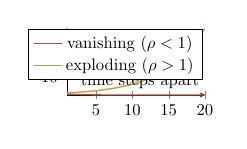
\begin{tikzpicture}[scale=0.6]
    \begin{axis}[width=4.5cm, height=3cm, xlabel=time steps apart, ylabel=gradient norm, domain=1:20, samples=50, axis lines=middle]
        \addplot[wp-primary, thick] {exp(-0.5*x)};
        \addplot[wp-accent, thick] {1.2^x};
        \legend{vanishing ($\rho<1$), exploding ($\rho>1$)};
    \end{axis}
\end{tikzpicture}
\caption{Exponential behaviour of gradient magnitude with sequence distance.}
\end{marginfigure}

The vanishing gradient problem is the primary reason simple RNNs cannot learn long‑range dependencies (e.g., more than 10–20 steps). Gated architectures (LSTM, GRU) mitigate this by allowing the gradient to bypass the multiplicative chain via additive updates.

\paragraph{Gradient Clipping}
When gradients explode, the parameter update becomes erratic and may cause overflow. A simple but effective remedy is \textbf{gradient clipping}. Two common variants exist:

\begin{defn}[Norm‑based Gradient Clipping]
    Let $\mathbf{g} = \nabla_{\boldsymbol{\theta}} \mathcal{L}$ be the gradient vector of all parameters. If $\|\mathbf{g}\| > c$, rescale it:
    \[
    \tilde{\mathbf{g}} = \frac{c}{\|\mathbf{g}\|} \mathbf{g}.
    \]
    Here $c > 0$ is a user‑defined threshold. This preserves the direction while bounding the step size.
\end{defn}

\begin{defn}[Value‑based Gradient Clipping]
    For each component $g_i$, set $\tilde{g}_i = \max(-c, \min(c, g_i))$. This is elementwise clipping.
\end{defn}

Norm clipping is preferred in RNNs because it respects the geometry of the parameter space. The following result guarantees stability:

\begin{thm}[Convergence with Clipping]
    Under standard assumptions (bounded gradients, Lipschitz loss), gradient clipping ensures that the parameter iterates remain bounded and that stochastic gradient descent converges almost surely to a stationary point, even when the unclipped gradients would diverge.
\end{thm}

In practice, $c$ is often set between $1$ and $5$ for RNNs. Clipping is applied before the parameter update.

\section{Gated Recurrent Architectures}

To mitigate the vanishing gradient problem, more sophisticated RNN cells introduce \textbf{gates} that control the flow of information.

\subsection{Long Short‑Term Memory (LSTM)}

The LSTM, proposed by Hochreiter and Schmidhuber (1997), maintains a separate cell state $\mathbf{c}_t$ in addition to the hidden state $\mathbf{h}_t$. The cell state acts as a “conveyor belt” that can carry information over many steps. Three gates control access:

\begin{itemize}
    \item \textbf{Forget gate}: $\mathbf{f}_t = \sigma(\mathbf{W}_f [\mathbf{h}_{t-1}, \mathbf{x}_t] + \mathbf{b}_f)$
    \item \textbf{Input gate}: $\mathbf{i}_t = \sigma(\mathbf{W}_i [\mathbf{h}_{t-1}, \mathbf{x}_t] + \mathbf{b}_i)$
    \item \textbf{Output gate}: $\mathbf{o}_t = \sigma(\mathbf{W}_o [\mathbf{h}_{t-1}, \mathbf{x}_t] + \mathbf{b}_o)$
\end{itemize}

A candidate cell update is $\tilde{\mathbf{c}}_t = \tanh(\mathbf{W}_c [\mathbf{h}_{t-1}, \mathbf{x}_t] + \mathbf{b}_c)$. Then the cell state and hidden state are updated:
\begin{align}
    \mathbf{c}_t &= \mathbf{f}_t \odot \mathbf{c}_{t-1} + \mathbf{i}_t \odot \tilde{\mathbf{c}}_t, \\
    \mathbf{h}_t &= \mathbf{o}_t \odot \tanh(\mathbf{c}_t).
\end{align}

The forget gate allows the network to selectively erase the past; the input gate decides which new information to store; the output gate controls what is exposed as the hidden state.

\subsection{Gated Recurrent Unit (GRU)}

The GRU (Cho et al., 2014) simplifies the LSTM by combining the forget and input gates into a single \textbf{update gate} and merging the cell and hidden states. Its equations are:
\begin{align}
    \mathbf{z}_t &= \sigma(\mathbf{W}_z [\mathbf{h}_{t-1}, \mathbf{x}_t] + \mathbf{b}_z) \quad \text{(update gate)}, \\
    \mathbf{r}_t &= \sigma(\mathbf{W}_r [\mathbf{h}_{t-1}, \mathbf{x}_t] + \mathbf{b}_r) \quad \text{(reset gate)}, \\
    \tilde{\mathbf{h}}_t &= \tanh(\mathbf{W}_h [\mathbf{r}_t \odot \mathbf{h}_{t-1}, \mathbf{x}_t] + \mathbf{b}_h), \\
    \mathbf{h}_t &= (1 - \mathbf{z}_t) \odot \mathbf{h}_{t-1} + \mathbf{z}_t \odot \tilde{\mathbf{h}}_t.
\end{align}
GRUs have fewer parameters than LSTMs and often perform similarly.

\begin{marginfigure}
\centering
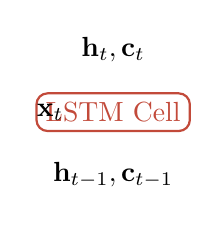
\begin{tikzpicture}[node distance=0.8cm, thick]
    \node[draw, rectangle, rounded corners, wp-primary] (lstm) {LSTM Cell};
    \node[above of=lstm] {$\mathbf{h}_t, \mathbf{c}_t$};
    \node[below of=lstm] {$\mathbf{h}_{t-1}, \mathbf{c}_{t-1}$};
    \node[left of=lstm] {$\mathbf{x}_t$};
\end{tikzpicture}
\caption{Schematic of an LSTM cell. The cell state $\mathbf{c}_t$ (not shown separately) flows through the top, modulated by gates.}
\end{marginfigure}

\subsection{Connection to Maximum Likelihood Estimation}

For sequence prediction (e.g., language modeling), the RNN defines a conditional probability distribution over the next token given the history:
\[
P(\mathbf{y}_t \mid \mathbf{x}_{1:t}, \mathbf{y}_{1:t-1}) = \text{softmax}(\mathbf{o}_t).
\]
The total likelihood of a sequence is $\prod_{t=1}^T P(\mathbf{y}_t \mid \text{history})$. Minimising the cross‑entropy loss is therefore equivalent to maximum likelihood estimation under the model.

\section{Practical Considerations and Extensions}

\begin{itemize}
    \item \textbf{Truncated BPTT}: For very long sequences, full BPTT is expensive. Truncated BPTT splits the sequence into blocks and only backpropagates a fixed number of steps ($k$) inside each block. This approximates the true gradient and is widely used.
    \item \textbf{Teacher forcing}: During training, the true previous target $\mathbf{y}_{t-1}$ (or a sample) is fed as input instead of the model’s own prediction. This speeds up training but may cause exposure bias.
    \item \textbf{Deep RNNs}: Stacking multiple RNN layers (each layer’s hidden state becomes input to the next layer) increases representational capacity.
    \item \textbf{Bidirectional RNNs}: Two RNNs process the sequence forward and backward, and their hidden states are concatenated. This provides context from both past and future, useful for sequence tagging.
\end{itemize}

\begin{algorithm}[h]
    \caption{Truncated BPTT (with block size $k$)}
    \begin{algorithmic}[1]
        \State Initialise $\mathbf{h}_0$.
        \For{each block $b$ of $k$ consecutive time steps}
            \State Run forward pass for $k$ steps, storing intermediate values.
            \State Compute loss for the block.
            \State Backpropagate gradients only through the $k$ steps (do not propagate beyond the block start).
            \State Update parameters.
            \State Carry over $\mathbf{h}_{b \cdot k}$ as initial state for the next block.
        \EndFor
    \end{algorithmic}
\end{algorithm}

\subsection{Attention Mechanisms}

A limitation of RNNs (even with gating) is that the fixed‑dimensional hidden state $\mathbf{h}_t$ must compress the entire history. For long sequences, this bottleneck causes information loss. Attention mechanisms overcome this by allowing the decoder to directly access all encoder hidden states.

\paragraph{Seq2Seq with Attention}
In a sequence‑to‑sequence model, an encoder RNN processes the input sequence $\mathbf{x}_{1:T}$ and produces hidden states $\mathbf{h}_1,\dots,\mathbf{h}_T$. A decoder RNN generates the output sequence $\mathbf{y}_{1:T'}$. At each decoder step $s$, an attention mechanism computes a context vector $\mathbf{c}_s$ as a weighted sum of encoder states:
\[
e_{s,t} = \text{score}(\mathbf{d}_{s-1}, \mathbf{h}_t),\quad
\alpha_{s,t} = \frac{\exp(e_{s,t})}{\sum_{t'=1}^T \exp(e_{s,t'})},\quad
\mathbf{c}_s = \sum_{t=1}^T \alpha_{s,t} \mathbf{h}_t.
\]
The score function is often additive (Bahdanau) or multiplicative (Luong). The context vector is then combined with the decoder’s hidden state to predict the next output.

\begin{defn}[Additive Attention]
    \[
    e_{s,t} = \mathbf{v}^{\mathsf{T}} \tanh(\mathbf{W}_d \mathbf{d}_{s-1} + \mathbf{W}_h \mathbf{h}_t + \mathbf{b}),
    \]
    where $\mathbf{v}, \mathbf{W}_d, \mathbf{W}_h, \mathbf{b}$ are learnable parameters.
\end{defn}

\begin{defn}[Multiplicative (Dot‑Product) Attention]
    \[
    e_{s,t} = \mathbf{d}_{s-1}^{\mathsf{T}} \mathbf{W} \mathbf{h}_t,
    \]
    where $\mathbf{W}$ is a learned matrix. If $\mathbf{W}$ is identity and norms are ignored, it becomes dot‑product attention.
\end{defn}

\begin{marginfigure}
\centering
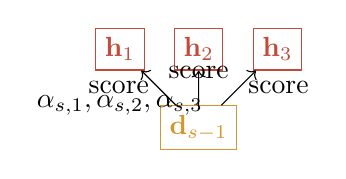
\begin{tikzpicture}[scale=0.6]
    \node[draw, rectangle, wp-primary] (enc1) {$\mathbf{h}_1$};
    \node[draw, rectangle, wp-primary, right of=enc1] (enc2) {$\mathbf{h}_2$};
    \node[draw, rectangle, wp-primary, right of=enc2] (enc3) {$\mathbf{h}_3$};
    \node[draw, rectangle, wp-accent, below of=enc2] (dec) {$\mathbf{d}_{s-1}$};
    \draw[->] (dec) -- node[left] {score} (enc1);
    \draw[->] (dec) -- node[above] {score} (enc2);
    \draw[->] (dec) -- node[right] {score} (enc3);
    \node at (0,-1.2) {$\alpha_{s,1},\alpha_{s,2},\alpha_{s,3}$};
\end{tikzpicture}
\caption{Attention aligns decoder state $\mathbf{d}_{s-1}$ with encoder states $\mathbf{h}_t$ to form a context vector.}
\end{marginfigure}

Attention has become the cornerstone of modern sequence models. In particular, the Transformer architecture replaces recurrence entirely with self‑attention, achieving state‑of‑the‑art results in machine translation, language modeling, and beyond. However, attention is also used inside RNNs to handle long sequences effectively.

\begin{thm}[Attention Bypasses Vanishing Gradients]
    The attention mechanism provides a direct gradient path from the decoder loss to each encoder hidden state, independent of the distance between them. This effectively solves the vanishing gradient problem for long‑range dependencies.
\end{thm}

\subsection{Regularization for Recurrent Networks}

Deep RNNs overfit easily, especially with small datasets. Standard dropout (applied to inputs or outputs) does not work well for recurrent connections because it corrupts the temporal signal. Specialized techniques have been developed.

\paragraph{Variational Dropout}
Proposed by Gal \& Ghahramani (2016), variational dropout applies the same dropout mask across all time steps for each recurrent connection. For a hidden state $\mathbf{h}_t$, the forward pass becomes:
\[
\mathbf{h}_t = \phi_h(\mathbf{W}_{hh}(\mathbf{m} \odot \mathbf{h}_{t-1}) + \mathbf{W}_{xh}\mathbf{x}_t + \mathbf{b}_h),
\]
where $\mathbf{m} \sim \text{Bernoulli}(p)$ is a fixed binary mask (same for all $t$). This is equivalent to a Bayesian interpretation of dropout as approximate variational inference in a deep Gaussian process.

\begin{marginfigure}
\centering
\begin{tikzpicture}[scale=0.6]
    \foreach \t in {1,2,3} {
        \node[draw, circle, wp-primary] (h\t) at (\t*1.5,0) {$h_{t}$};
        \node[draw, circle, wp-muted] (x\t) at (\t*1.5,-1) {$x_t$};
        \draw[->] (x\t) -- (h\t);
        \ifnum\t>1 \draw[->] (h\prev) -- (h\t); \fi
        \node at (\t*1.5,0.5) {$\times \mathbf{m}$};
    }
\end{tikzpicture}
\caption{Variational dropout: same mask $\mathbf{m}$ applied at every time step.}
\end{marginfigure}

\paragraph{Zoneout}
Zoneout (Krueger et al., 2017) stochastically replaces the computed hidden state with the previous hidden state:
\[
\mathbf{h}_t = \mathbf{z}_t \odot \phi_h(\mathbf{W}_{hh}\mathbf{h}_{t-1} + \mathbf{W}_{xh}\mathbf{x}_t + \mathbf{b}_h) + (1 - \mathbf{z}_t) \odot \mathbf{h}_{t-1},
\]
where $\mathbf{z}_t \sim \text{Bernoulli}(p)$. This preserves information flow and helps with vanishing gradients.

\paragraph{Layer Normalization for RNNs}
Layer normalization (Ba et al., 2016) normalises the pre‑activation across the feature dimension:
\[
\mu_t = \frac{1}{d_h}\sum_{i=1}^{d_h} a_{t,i},\quad \sigma_t^2 = \frac{1}{d_h}\sum_{i=1}^{d_h} (a_{t,i} - \mu_t)^2,\quad \tilde{\mathbf{a}}_t = \frac{\mathbf{a}_t - \mu_t}{\sqrt{\sigma_t^2 + \epsilon}},\quad \mathbf{h}_t = \phi_h(\gamma \tilde{\mathbf{a}}_t + \beta).
\]
It stabilises training and is especially effective with LSTMs.

\begin{remark}
    In practice, a combination of variational dropout on recurrent connections and layer normalization is often used in state‑of‑the‑art RNNs (e.g., AWD‑LSTM).
\end{remark}

\subsection{Probabilistic Recurrent Neural Networks}

Deterministic RNNs map a deterministic input sequence to a deterministic hidden state. For uncertainty quantification and generative modeling, we introduce **stochastic latent variables**.

\paragraph{Variational RNN (VRNN)}
The VRNN (Chung et al., 2015) augments the RNN hidden state with a latent variable $\mathbf{z}_t$ at each time step. The generative model is:
\begin{align}
    \mathbf{h}_{t-1} &= f(\mathbf{x}_{t-1}, \mathbf{z}_{t-1}, \mathbf{h}_{t-2}), \\
    \mathbf{z}_t &\sim \mathcal{N}(\boldsymbol{\mu}_{z,t}, \operatorname{diag}(\boldsymbol{\sigma}_{z,t}^2)), \quad \text{where } [\boldsymbol{\mu}_{z,t}, \log \boldsymbol{\sigma}_{z,t}^2] = \psi(\mathbf{h}_{t-1}), \\
    \mathbf{x}_t &\sim \mathcal{N}(\boldsymbol{\mu}_{x,t}, \operatorname{diag}(\boldsymbol{\sigma}_{x,t}^2)), \quad \text{where } [\boldsymbol{\mu}_{x,t}, \log \boldsymbol{\sigma}_{x,t}^2] = \theta(\mathbf{h}_{t-1}, \mathbf{z}_t).
\end{align}
The inference (posterior) network approximates $q(\mathbf{z}_t \mid \mathbf{x}_{\le t}, \mathbf{h}_{t-1})$ with parameters from a neural network $\phi$.

The training objective is the sequential evidence lower bound (ELBO):
\[
\mathcal{L} = \sum_{t=1}^T \mathbb{E}_{q(\mathbf{z}_t \mid \cdot)} \bigl[ \log p(\mathbf{x}_t \mid \mathbf{z}_t, \mathbf{h}_{t-1}) \bigr] - \operatorname{KL}\bigl( q(\mathbf{z}_t \mid \mathbf{x}_{\le t}, \mathbf{h}_{t-1}) \| p(\mathbf{z}_t \mid \mathbf{h}_{t-1}) \bigr).
\]

\begin{marginfigure}
\centering
\begin{tikzpicture}[node distance=0.8cm, thick]
    \node[draw, circle, wp-primary] (z1) {$\mathbf{z}_1$};
    \node[draw, circle, wp-primary, right of=z1] (z2) {$\mathbf{z}_2$};
    \node[draw, circle, wp-primary, right of=z2] (z3) {$\mathbf{z}_3$};
    \node[draw, circle, wp-accent, below of=z1] (h0) {$\mathbf{h}_0$};
    \node[draw, circle, wp-accent, right of=h0] (h1) {$\mathbf{h}_1$};
    \node[draw, circle, wp-accent, right of=h1] (h2) {$\mathbf{h}_2$};
    \draw[->] (z1) -- (h1); \draw[->] (z2) -- (h2); \draw[->] (z3) -- (h3);
    \draw[->] (h0) -- (z1); \draw[->] (h1) -- (z2); \draw[->] (h2) -- (z3);
    \draw[->] (h0) -- (h1); \draw[->] (h1) -- (h2);
    \node at (0,-1.2) {VRNN graphical model};
\end{tikzpicture}
\caption{VRNN: deterministic RNN hidden states $\mathbf{h}_t$ and stochastic latents $\mathbf{z}_t$ interact.}
\end{marginfigure}

VRNNs can generate highly structured sequences (e.g., handwriting, speech) and quantify predictive uncertainty.

\subsection{Memory Augmented RNNs}

Standard RNNs compress all history into a fixed‑dimensional hidden state, which limits long‑term memory. Memory augmented networks introduce an external memory matrix that the RNN can read from and write to.

\begin{defn}[Neural Turing Machine (NTM)]
    An NTM consists of:
    \begin{itemize}
        \item A controller (RNN) that outputs read/write vectors.
        \item A memory matrix $\mathbf{M}_t \in \mathbb{R}^{N \times M}$ (size $N$ vectors of dimension $M$).
        \item Read heads produce content‑based and location‑based addressing.
    \end{itemize}
    At each step, the controller reads $\mathbf{r}_t = \sum_i \alpha_i^{\text{read}} \mathbf{M}_t[i,:]$, where $\boldsymbol{\alpha}^{\text{read}}$ is an attention distribution.
    Writing combines an erase vector $\mathbf{e}_t$ and an add vector $\mathbf{a}_t$:
    \[
    \mathbf{M}_{t+1}[i,:] = \mathbf{M}_t[i,:] \odot (1 - \alpha_i^{\text{write}} \mathbf{e}_t) + \alpha_i^{\text{write}} \mathbf{a}_t.
    \]
\end{defn}

The **Differentiable Neural Computer (DNC)** (Graves et al., 2016) extends the NTM with dynamic memory allocation and temporal linking, enabling it to solve complex algorithmic tasks like graph traversal and reasoning.

\begin{marginfigure}
\centering
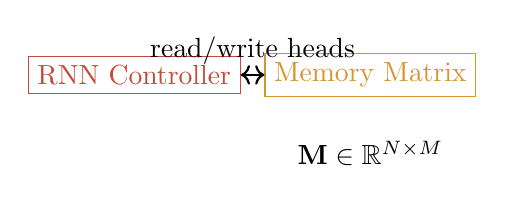
\begin{tikzpicture}[scale=0.5]
    \node[draw, rectangle, wp-primary] (ctrl) {RNN Controller};
    \node[draw, rectangle, wp-accent, right of=ctrl, node distance=3cm] (mem) {Memory Matrix};
    \draw[<->, thick] (ctrl) -- node[above] {read/write heads} (mem);
    \node[below of=mem] {$\mathbf{M} \in \mathbb{R}^{N \times M}$};
\end{tikzpicture}
\caption{Neural Turing Machine: an RNN controller accesses an external memory matrix.}
\end{marginfigure}

Memory augmented RNNs can learn to copy long sequences, sort numbers, and perform reasoning tasks that standard RNNs fail at. However, they are more computationally expensive and harder to train.

\subsection{Graph Recurrent Neural Networks}

When data are graphs (e.g., molecules, social networks), sequential ordering is not natural. Graph RNNs generalise the recurrence to propagation over graph edges.

\begin{defn}[Gated Graph Neural Network (GGNN)]
    For a graph with nodes $v \in \mathcal{V}$, each node has a hidden state $\mathbf{h}_v^{(t)}$ that evolves according to:
    \[
    \mathbf{a}_v^{(t)} = \sum_{u \in \mathcal{N}(v)} \mathbf{W}_{vu} \mathbf{h}_u^{(t-1)} + \mathbf{W}_x \mathbf{x}_v,
    \]
    where $\mathcal{N}(v)$ are neighbours of $v$. The state update uses a GRU cell:
    \[
    \mathbf{h}_v^{(t)} = \text{GRU}(\mathbf{h}_v^{(t-1)}, \mathbf{a}_v^{(t)}).
    \]
    After $T$ steps, the final node states are used for predictions (e.g., graph classification).
\end{defn}

GGNNs are a special case of message‑passing neural networks. They can handle cycles and learn long‑range dependencies on graphs.

\begin{marginfigure}
\centering
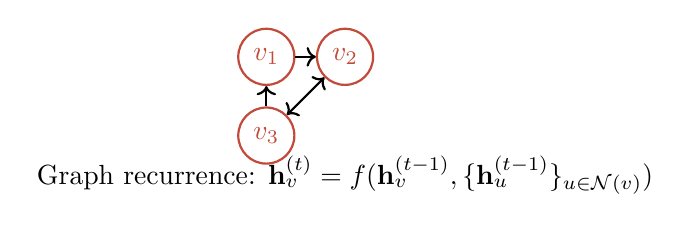
\begin{tikzpicture}[node distance=1cm, thick]
    \node[draw, circle, wp-primary] (v1) {$v_1$};
    \node[draw, circle, wp-primary, right of=v1] (v2) {$v_2$};
    \node[draw, circle, wp-primary, below of=v1] (v3) {$v_3$};
    \draw[->] (v3) -- (v1); \draw[->] (v1) -- (v2); \draw[<->] (v2) -- (v3);
    \node at (1, -1.5) {Graph recurrence: $\mathbf{h}_{v}^{(t)} = f(\mathbf{h}_{v}^{(t-1)}, \{\mathbf{h}_u^{(t-1)}\}_{u \in \mathcal{N}(v)})$};
\end{tikzpicture}
\caption{In a Graph RNN, each node’s state is updated using messages from neighbours.}
\end{marginfigure}

\subsection{Continuous‑Time RNNs: Neural ODEs}

Standard RNNs assume a discrete time index. Neural ODEs (Chen et al., 2018) treat the hidden state as a continuous function of time.

\begin{defn}[ODE‑RNN]
    The hidden state evolution is governed by an ordinary differential equation:
    \[
    \frac{d\mathbf{h}(t)}{dt} = f_\theta(\mathbf{h}(t), \mathbf{x}(t)),
    \]
    where $\mathbf{x}(t)$ is a continuous‑time input (e.g., interpolated from discrete observations). The state at observation times is obtained by integration:
    \[
    \mathbf{h}(t_n) = \mathbf{h}(t_{n-1}) + \int_{t_{n-1}}^{t_n} f_\theta(\mathbf{h}(\tau), \mathbf{x}(\tau)) \, d\tau.
    \]
\end{defn}

This formulation naturally handles irregularly sampled time series. The adjoint sensitivity method allows backpropagation through the ODE solver without storing all intermediate states, reducing memory usage.

\begin{marginfigure}
\centering
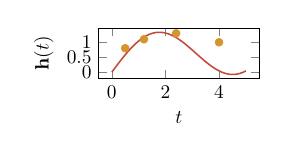
\begin{tikzpicture}[scale=0.7]
    \begin{axis}[width=4.5cm, height=2.5cm, xlabel=$t$, ylabel=$\mathbf{h}(t)$, domain=0:5, samples=100]
        \addplot[wp-primary, thick] {sin(deg(x)) + 0.2*x};
        \addplot[only marks, mark=*, wp-accent] coordinates {(0.5,0.8) (1.2,1.1) (2.4,1.3) (4.0,1.0)};
    \end{axis}
\end{tikzpicture}
\caption{Continuous hidden state $\mathbf{h}(t)$ (line) with discrete observations (dots) at irregular times.}
\end{marginfigure}

Connection to RNNs: An RNN can be seen as a discretisation of an ODE using a simple Euler step:
\[
\mathbf{h}_t - \mathbf{h}_{t-1} = f_\theta(\mathbf{h}_{t-1}, \mathbf{x}_t).
\]
Neural ODEs replace the fixed step with an adaptive ODE solver, providing a more flexible and theoretically grounded model for continuous‑time dynamics.

\subsection{Evaluation Metrics for Sequence Models}

Measuring performance of sequence models depends on the task. Below are the most common metrics with formal definitions.

\paragraph{Perplexity (Language Models)}
Given a test sequence $y_{1:T}$ and a model predicting $P(y_t \mid y_{<t})$, perplexity is
\[
\text{PPL} = \exp\left(-\frac{1}{T}\sum_{t=1}^T \log P(y_t \mid y_{<t})\right).
\]
Lower perplexity indicates better generalisation. For a uniform model over a vocabulary of size $V$, PPL $= V$.

\paragraph{Word Error Rate (WER) (Speech Recognition)}
WER is the edit distance (Levenshtein) between the predicted word sequence $\hat{\mathbf{w}}$ and the reference $\mathbf{w}$, normalised by the reference length:
\[
\text{WER} = \frac{\text{Insertions} + \text{Deletions} + \text{Substitutions}}{|\mathbf{w}|}.
\]

\paragraph{BLEU Score (Machine Translation)}
BLEU measures $n$-gram overlap between candidate and reference translations with a brevity penalty (BP):
\[
\text{BLEU} = \text{BP} \cdot \exp\left(\sum_{n=1}^N w_n \log p_n\right),\quad
p_n = \frac{\text{\# of $n$-grams in candidate that appear in reference}}{\text{\# of $n$-grams in candidate}}.
\]
Typically $N=4$ and $w_n = 1/N$.

\paragraph{ROUGE (Summarisation)}
ROUGE (Recall‑Oriented Understudy for Gisting Evaluation) computes recall of $n$-grams and longest common subsequences. ROUGE‑N is $n$-gram recall: $\frac{\sum_{n\text{-gram} \in \text{ref}} \min(\text{count}_{\text{ref}}, \text{count}_{\text{cand}})}{\sum_{n\text{-gram} \in \text{ref}} \text{count}_{\text{ref}}}$.

\begin{remark}
    No single metric captures all aspects of quality. BLEU correlates weakly with human judgment; newer metrics like BERTScore (using contextual embeddings) are gaining popularity.
\end{remark}

\subsection{Autoregressive Sequence Generation}

Once an RNN is trained, we can generate new sequences by sampling from the learned conditional distribution. This is an \textbf{autoregressive} process: each new token is generated based on previously generated tokens.

\paragraph{Greedy Decoding}
At each step $t$, choose $\hat{y}_t = \arg\max P(y_t \mid \text{history})$. This is fast but can lead to repetitive or suboptimal sequences.

\paragraph{Beam Search}
Maintain a set of $k$ (beam width) best candidate sequences. At each step, expand each candidate by all possible next tokens, keep the top $k$ overall. Beam search often produces higher‑quality outputs.

\paragraph{Sampling with Temperature}
The output softmax distribution is often sharpened or flattened using a temperature parameter $\tau$:
\[
P(y_t = i \mid \text{history}) = \frac{\exp(z_i / \tau)}{\sum_j \exp(z_j / \tau)},
\]
where $z_i$ are the pre‑softmax logits. For $\tau \to 0$, sampling approaches greedy (deterministic); for $\tau = 1$, we recover the original distribution; for $\tau \to \infty$, the distribution becomes uniform. This controls the “creativity” of the generated text.

\begin{exmp}[Character‑Level RNN Sampling]
    A character RNN trained on Shakespeare can generate new text by starting with a seed character, then repeatedly sampling the next character from the predicted distribution (with, say, $\tau = 0.8$). The generated text often mimics the style of the original corpus.
\end{exmp}

\begin{marginfigure}
\centering
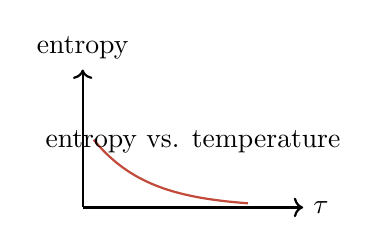
\begin{tikzpicture}[scale=0.7]
    \draw[->, thick] (0,0) -- (4,0) node[right] {$\tau$};
    \draw[->, thick] (0,0) -- (0,2.5) node[above] {entropy};
    \draw[wp-primary, thick, domain=0.2:3, samples=50] plot (\x, {1.5*exp(-\x)});
    \node at (2,1.2) {entropy vs. temperature};
\end{tikzpicture}
\caption{As temperature $\tau$ increases, the sampling distribution becomes more uniform (higher entropy).}
\end{marginfigure}


\subsection{Open Problems and Limitations of RNNs}

Despite their success, RNNs have fundamental limitations that remain active research areas.

\paragraph{Turing Completeness and Precision}
Siegelmann \& Sontag (1995) proved that RNNs with rational weights are Turing‑complete. However, this requires infinite precision. In practice, finite precision limits memory capacity; an RNN with $d_h$ hidden units can only store $\mathcal{O}(d_h \log d_h)$ bits of information, making it impossible to emulate arbitrary long‑range dependencies beyond a certain length.

\paragraph{The Expressivity vs. Trainability Tradeoff}
Deep (stacked) RNNs can represent complex functions, but they suffer from vanishing/exploding gradients even with gating. While LSTMs and GRUs alleviate the issue for sequences of hundreds of steps, they still struggle with dependencies spanning thousands of steps (e.g., language modeling over full books). Attention mechanisms largely solve this but move away from recurrence.

\paragraph{Orthogonal and Unitary RNNs}
To enforce gradient preservation, researchers have constrained $\mathbf{W}_{hh}$ to be orthogonal or unitary (where eigenvalues lie on the unit circle). Such RNNs guarantee that the Jacobian norm is exactly $1$, eliminating vanishing/exploding gradients. However, they are less expressive than full RNNs and training is constrained.

\begin{thm}[Unitary RNN Gradient Flow]
    If $\mathbf{W}_{hh}$ is unitary ($\mathbf{W}_{hh}^{\mathsf{H}} \mathbf{W}_{hh} = \mathbf{I}$) and $\phi_h$ is identity, then $\|\frac{\partial \mathbf{h}_t}{\partial \mathbf{h}_{t-k}}\| = 1$ for all $k$.
\end{thm}

\paragraph{The Fundamental Bottleneck of Fixed‑Size Hidden States}
No matter how many units, a fixed‑size hidden state cannot store unlimited information. This is the justification for external memory (NTM/DNC) and attention (which accesses all past states). However, attention has quadratic cost in sequence length, leading to the current research frontier: efficient transformers and linear RNNs (e.g., RWKV, S4).

\paragraph{Recurrent vs. Convolutional vs. Transformer Tradeoffs}
\begin{itemize}
    \item RNNs: linear time and memory in $T$, but weak long‑range memory.
    \item CNNs (e.g., WaveNet): parallel training, but require many layers for long‑range dependencies.
    \item Transformers: excellent long‑range memory, but quadratic cost (addressed by sparse attention, linear attention).
\end{itemize}
No single architecture dominates all regimes; the choice depends on sequence length, hardware, and task structure.


\section{Summary}

Recurrent Neural Networks provide a principled framework for modeling sequential data by maintaining an internal state that evolves over time. The training procedure, backpropagation through time, is a direct extension of the backpropagation algorithm for feedforward networks but must handle weight sharing across time. The vanishing and exploding gradient problems are inherent to simple RNNs; gated architectures (LSTM, GRU) are the standard solution. These models form the basis of modern sequence‑to‑sequence learning, machine translation, speech recognition, and many other applications.

The mathematical tools developed in earlier chapters – probability, MLE, gradient descent, and information theory – all play a role in understanding and training RNNs. The next logical step is to explore attention mechanisms and transformers, which have largely replaced RNNs in many domains but still rely on the same foundational concepts.

\end{document}